\documentclass[../../main.tex]{subfiles}

\newcommand{\NN}{\ensuremath{\mathrm{N}_{2}}}
\newcommand{\HH}{\ensuremath{\mathrm{H}_{2}}}

\newcommand{\CN}{\mbox{CEDAR-N}}
\newcommand{\CW}{\mbox{CEDAR-W}}
\newcommand{\CH}{\mbox{CEDAR-H}}


\begin{document}
    CEDARs were designed and built at CERN to detect secondary beam particles at the Super Proton Synchrotron (SPS). Two types of CEDAR were developed at CERN:
    CEDAR-W and CEDAR-N, corresponding to the areas of use. The two designs differ in terms of energy range in which they can detect beam particles, with CEDAR-N 
    able to separate kaons and pions up to $300 GeV / c$ but not detect protons below $60 GeV / c$. Whereas CEDAR-W can detect protons down to $12 GeV / c$ 
    and separate kaons and pions up to $150 GeV / c$. 
    %% Describe the previous performace of CEDAR-W with Nitrogen
    \newline\indent Described in section \_\_, NA62 has run with a CEDAR-W since 2016 filled with Nitrogen (\NN\) at a pressure of 1.71\,bar (absolute pressure).
    In this configuration, the CEDAR contributed to the most significant amount of material in the path of the beam, introducing $39 \times 10^{-3}\,X_0$ of material, 
    where $X_0$ is one radiation length. The aluminum windows of the CEDAR vessel contribute $3.9 \times 10^{-3}\,X_0$ and the \NN\ gas contributes $35 \times 10^{-3}\,X_0$.
    The material from the \CW\ with \NN\ results in multiple scattering of beam particles, which introduces an angular divergence of $32\,\mu rad$. Scattered beam particles 
    contribute to the backgrounds for the searches for ultra-rare decays, so it is imperative to reduce the amount of material in the beam to control these backgrounds. 
    It was proposed that a CEDAR filled with Hydrogen (\HH) could reduce the material due to the radiator gas. Using \HH\ as a radiator gas would require a pressure of 3.8\,bar 
    to produce a similar Cherenkov angle as \NN at 1.71\bar, which would instead introduce $3.4 \times 10^{-3}\,X_0$ of material. This would result in a $21\,\%$ reduction in total 
    material to $7.3 \times 10^{-3}\,X_0$. Resulting in an anglar beam divergence of $13\,\mu rad$ in both the horizontal and vertical dimensions. 

    \newline\indent Taking into account that the four GTk stations contribute $20 \times 10^{-3}\,X_0$, the total beam material along the beam-line reduces from $59 \times 10^{-3}\,X_0$ 
    to $27 \times 10^{-3}\,X_0$. Using the full NA62 simulation based on GEANT4, it is possible to estimate that the number of particles interacting inelastically and elastically upstream 
    of the decay volume would reduce from $2.1\,\%$ to $0.9\,\%$ (DO THIS YOUR SELF TO CHECK). This reduction in scattering would result in higher kaon transmission (number of kaons reaching the
    decay volume) and reduce the signal rates in downstream detectors. %%% May be we can add things about trigger rates but I think we should do a quick study

    \section{CEDAR description}
    
    \begin{figure}[t]
        \centering 
        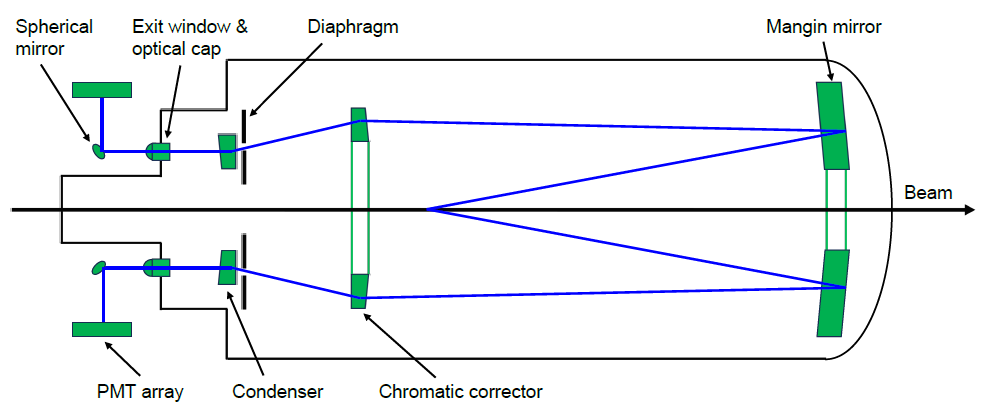
\includegraphics[width=0.8\textwidth]{imgs/cedar_diagram.png}
        \linespread{1.0}
        \caption{Diagram showing the optics of the CEDAR and KTAG in green as well as expected Cherenkov ring path in blue}
        \label{fig:ManginReflec}
    \end{figure}
    A CEDAR comprises a thermally insulated gas vessel comprising of two sections: a 4.3\,m long cylinder with an inner diameter of 53\,cm and a vessel cap 
    which can differ in length, depending on the CEDAR variant. The CEDAR-W has a vessel cap of 34\,cm long, with the CEDAR-N's being 28\,cm long and is attached to the main cylinder 
    at the upstream end. The gas vessel is separated from the vacuum of the beam-pipe by two aluminum windows at the upstream and downstream end. 
    \newline\indent The beam is designed to pass through the CEDAR vessel along the longitudinal access, passing through the radiator gas. When the beam passes through the vessel Cherenkov
    light is produced with an angle dependent on the mass and momentum of the beam particle and is defined as equation \ref{eq:Cherenkov2}.
    \begin{equation}\label{eq:Cherenkov2}
        cos(\theta) = \frac{1}{\beta n}
    \end{equation}
    The CEDAR contains optics inside the vessel connected to supports to allow the focusing of the produced Cherenkov light to reach the diaphragm at a radius of 100\,mm. 
    The light produced is reflected back upstream by a Mangin mirror \cite{Riedl:74}, which is a mirror comprising of two spherical surfaces with the dowstream lense cemented onto a concave mirror. The 
    mirror was designed to reduce any spheical aberrations, which is an effect intrinsic to lenses and curved mirrors where the light that strikes the spherical surface off-center is refracted/reflected
    vary compared to the light that strikes the center. After the mirror is a plano-convex lens called the Chromatic Corrector, which is designed in such a way that it corrects for the chromatic dispersion of the radiator gas
    and directs the light towards the diaphragm.
    This is where the different wavelengths of light refract differently in a medium, causing the ring to disperse, which would cause issues when it reaches the small diaphragm opening. Both the Mangin mirror and the 
    Chromatic corrector have a hole in the center to allow for the beam to pass through without impacting the optics. 
    
    \newline\indent The diaphragm shown in figure \ref{fig:cedarpics}, is a disk with eight seperate aperatures. Each aperature has an inner and outer element which allows the aperture to open as wide as 
    20\,mm and closed to 0\,mm. These elements can be seen in Figure \ref{fig:cedarpics} (right), where the aperture is set at a small value only to select a single Cherenkov ring of radius 100\,mm.  
    The mechanism is operated by a stepper motor connected to the shaft shown in figure \ref{fig:cedarpics} (left), where turning the shaft clockwise opens the diaphragm and the opposite closes it. The 
    shaft is also connected to a potentiometer that measures the rotation, which can then be converted to an aperture in millimeters. A pair of end switches are in place to alert the user if the aperture 
    is fully open or fully closed, which is essential so as not to cause any damage to the mechanical system.
    
    \begin{figure}[t]
        \centering
        \subfloat{{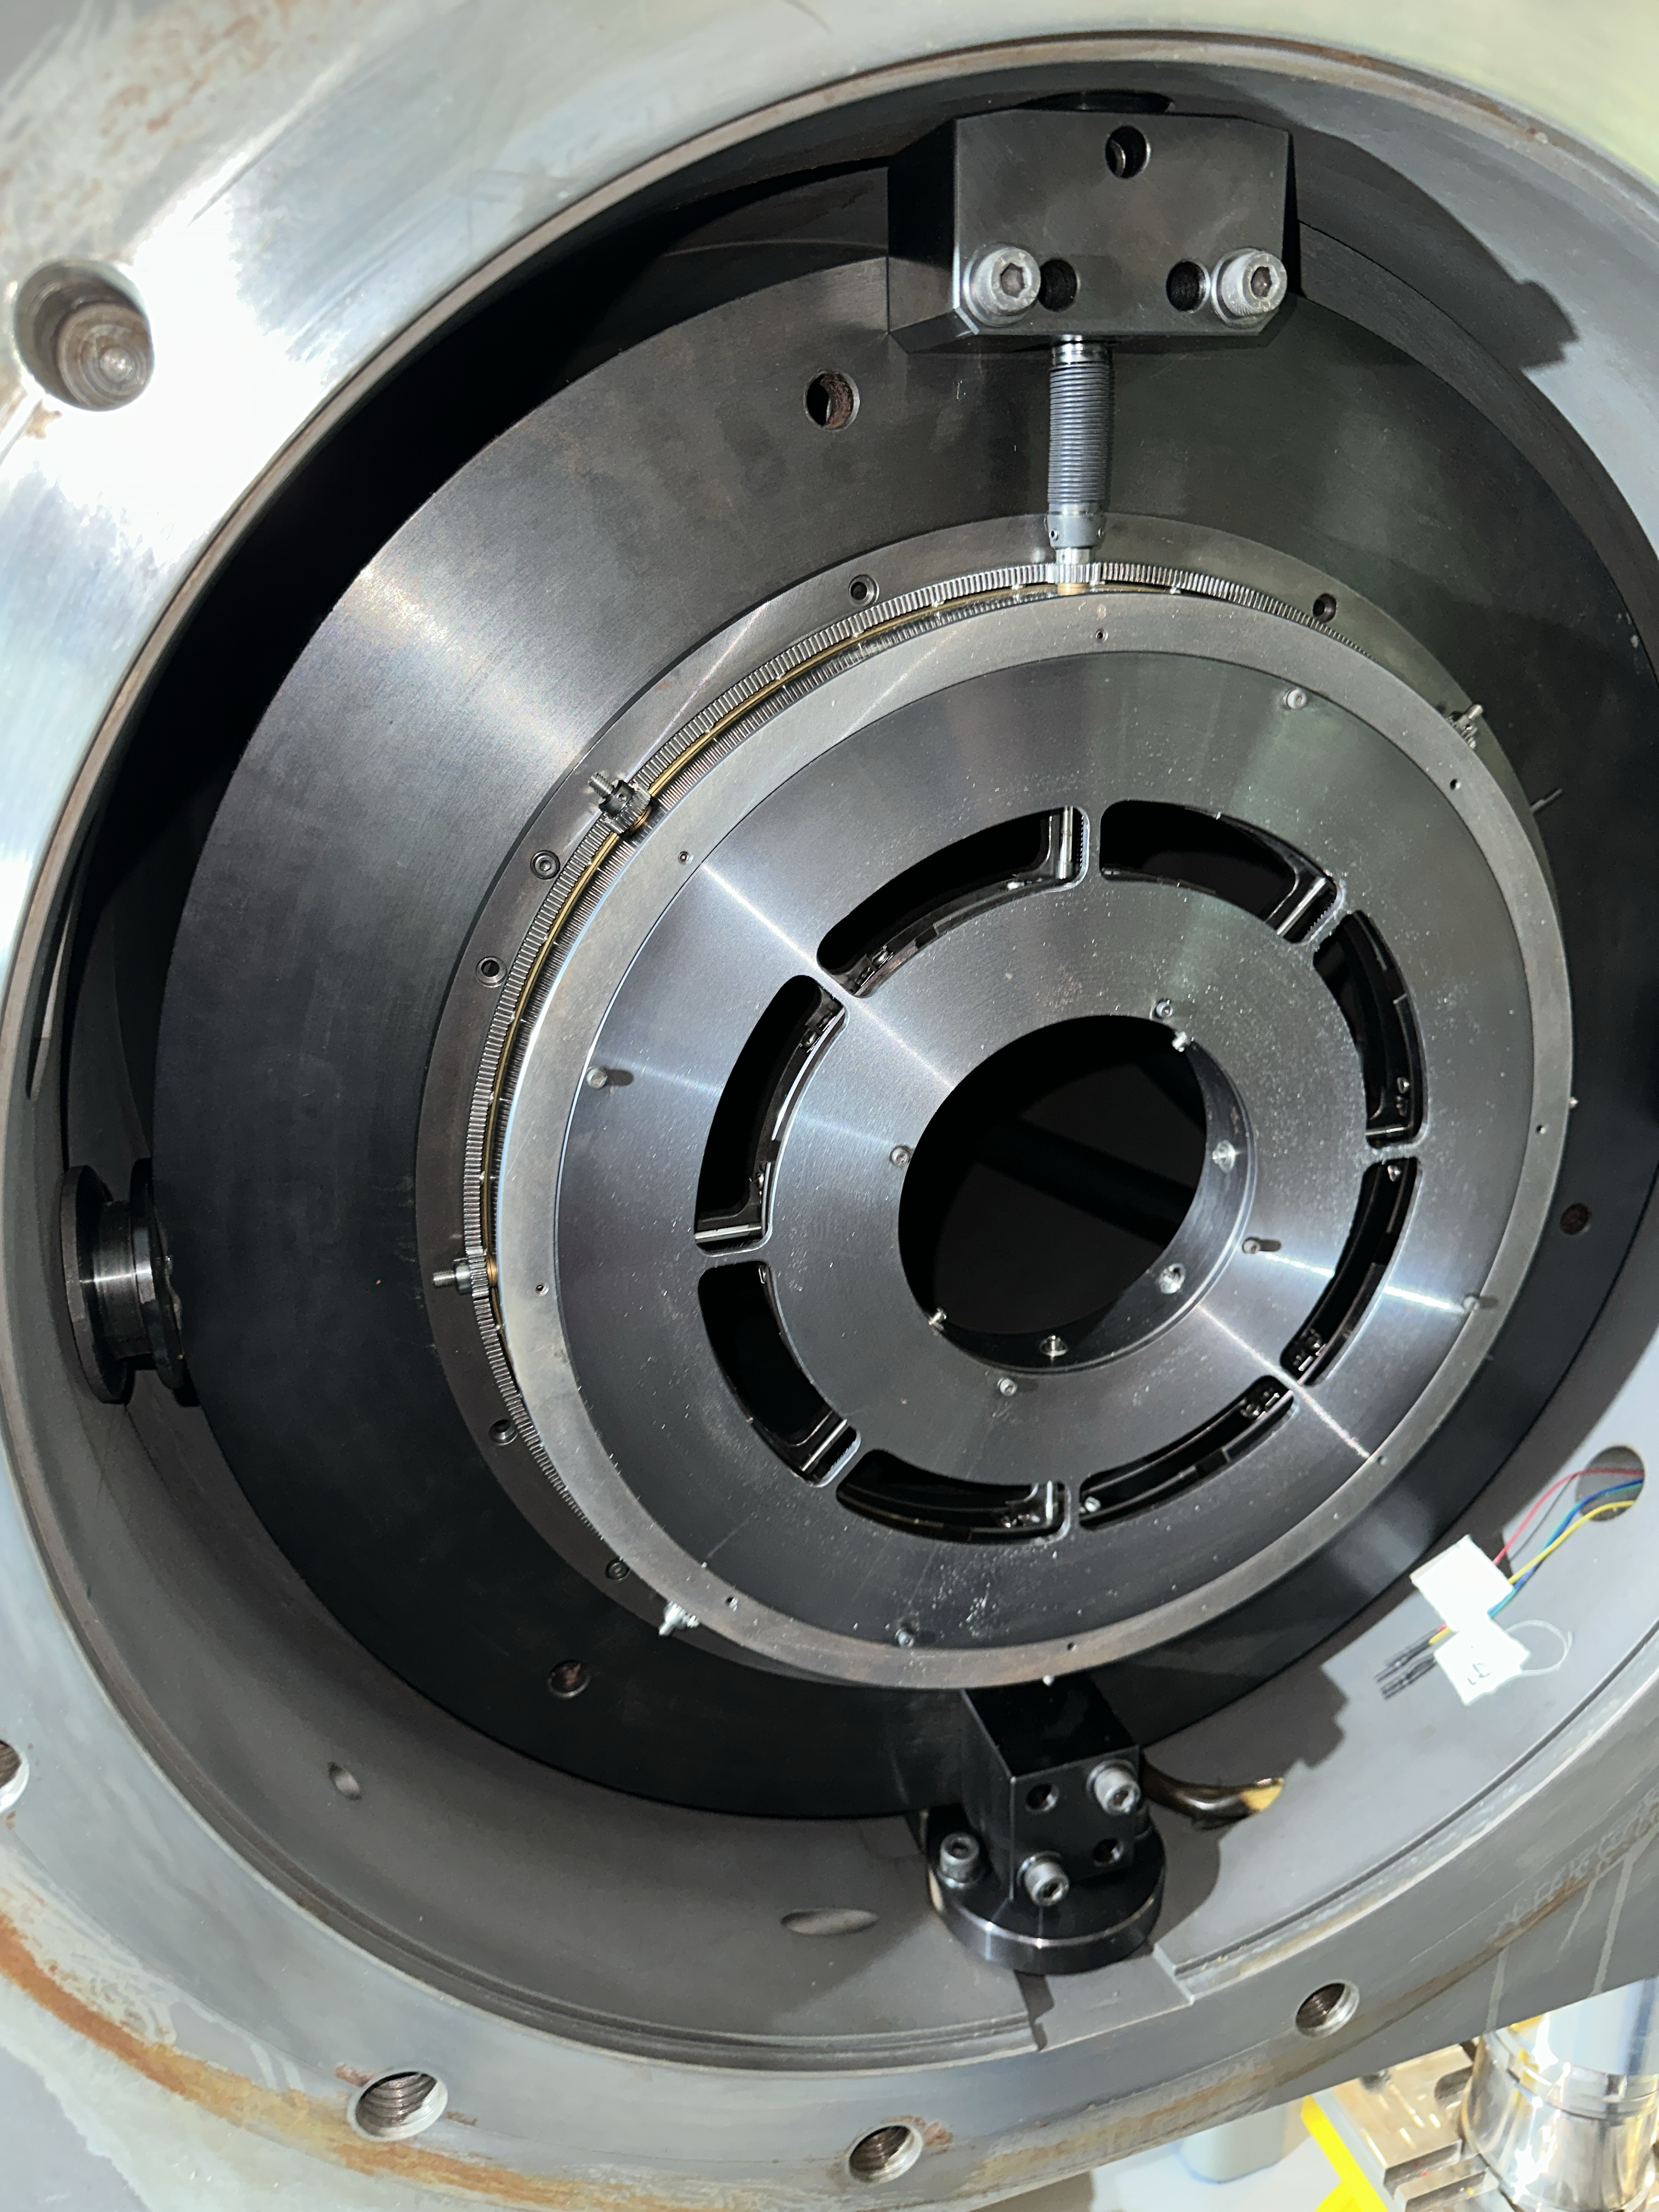
\includegraphics[height=8cm, width=0.5\textwidth]{imgs/Diaphragm.png} }}%
        \subfloat{{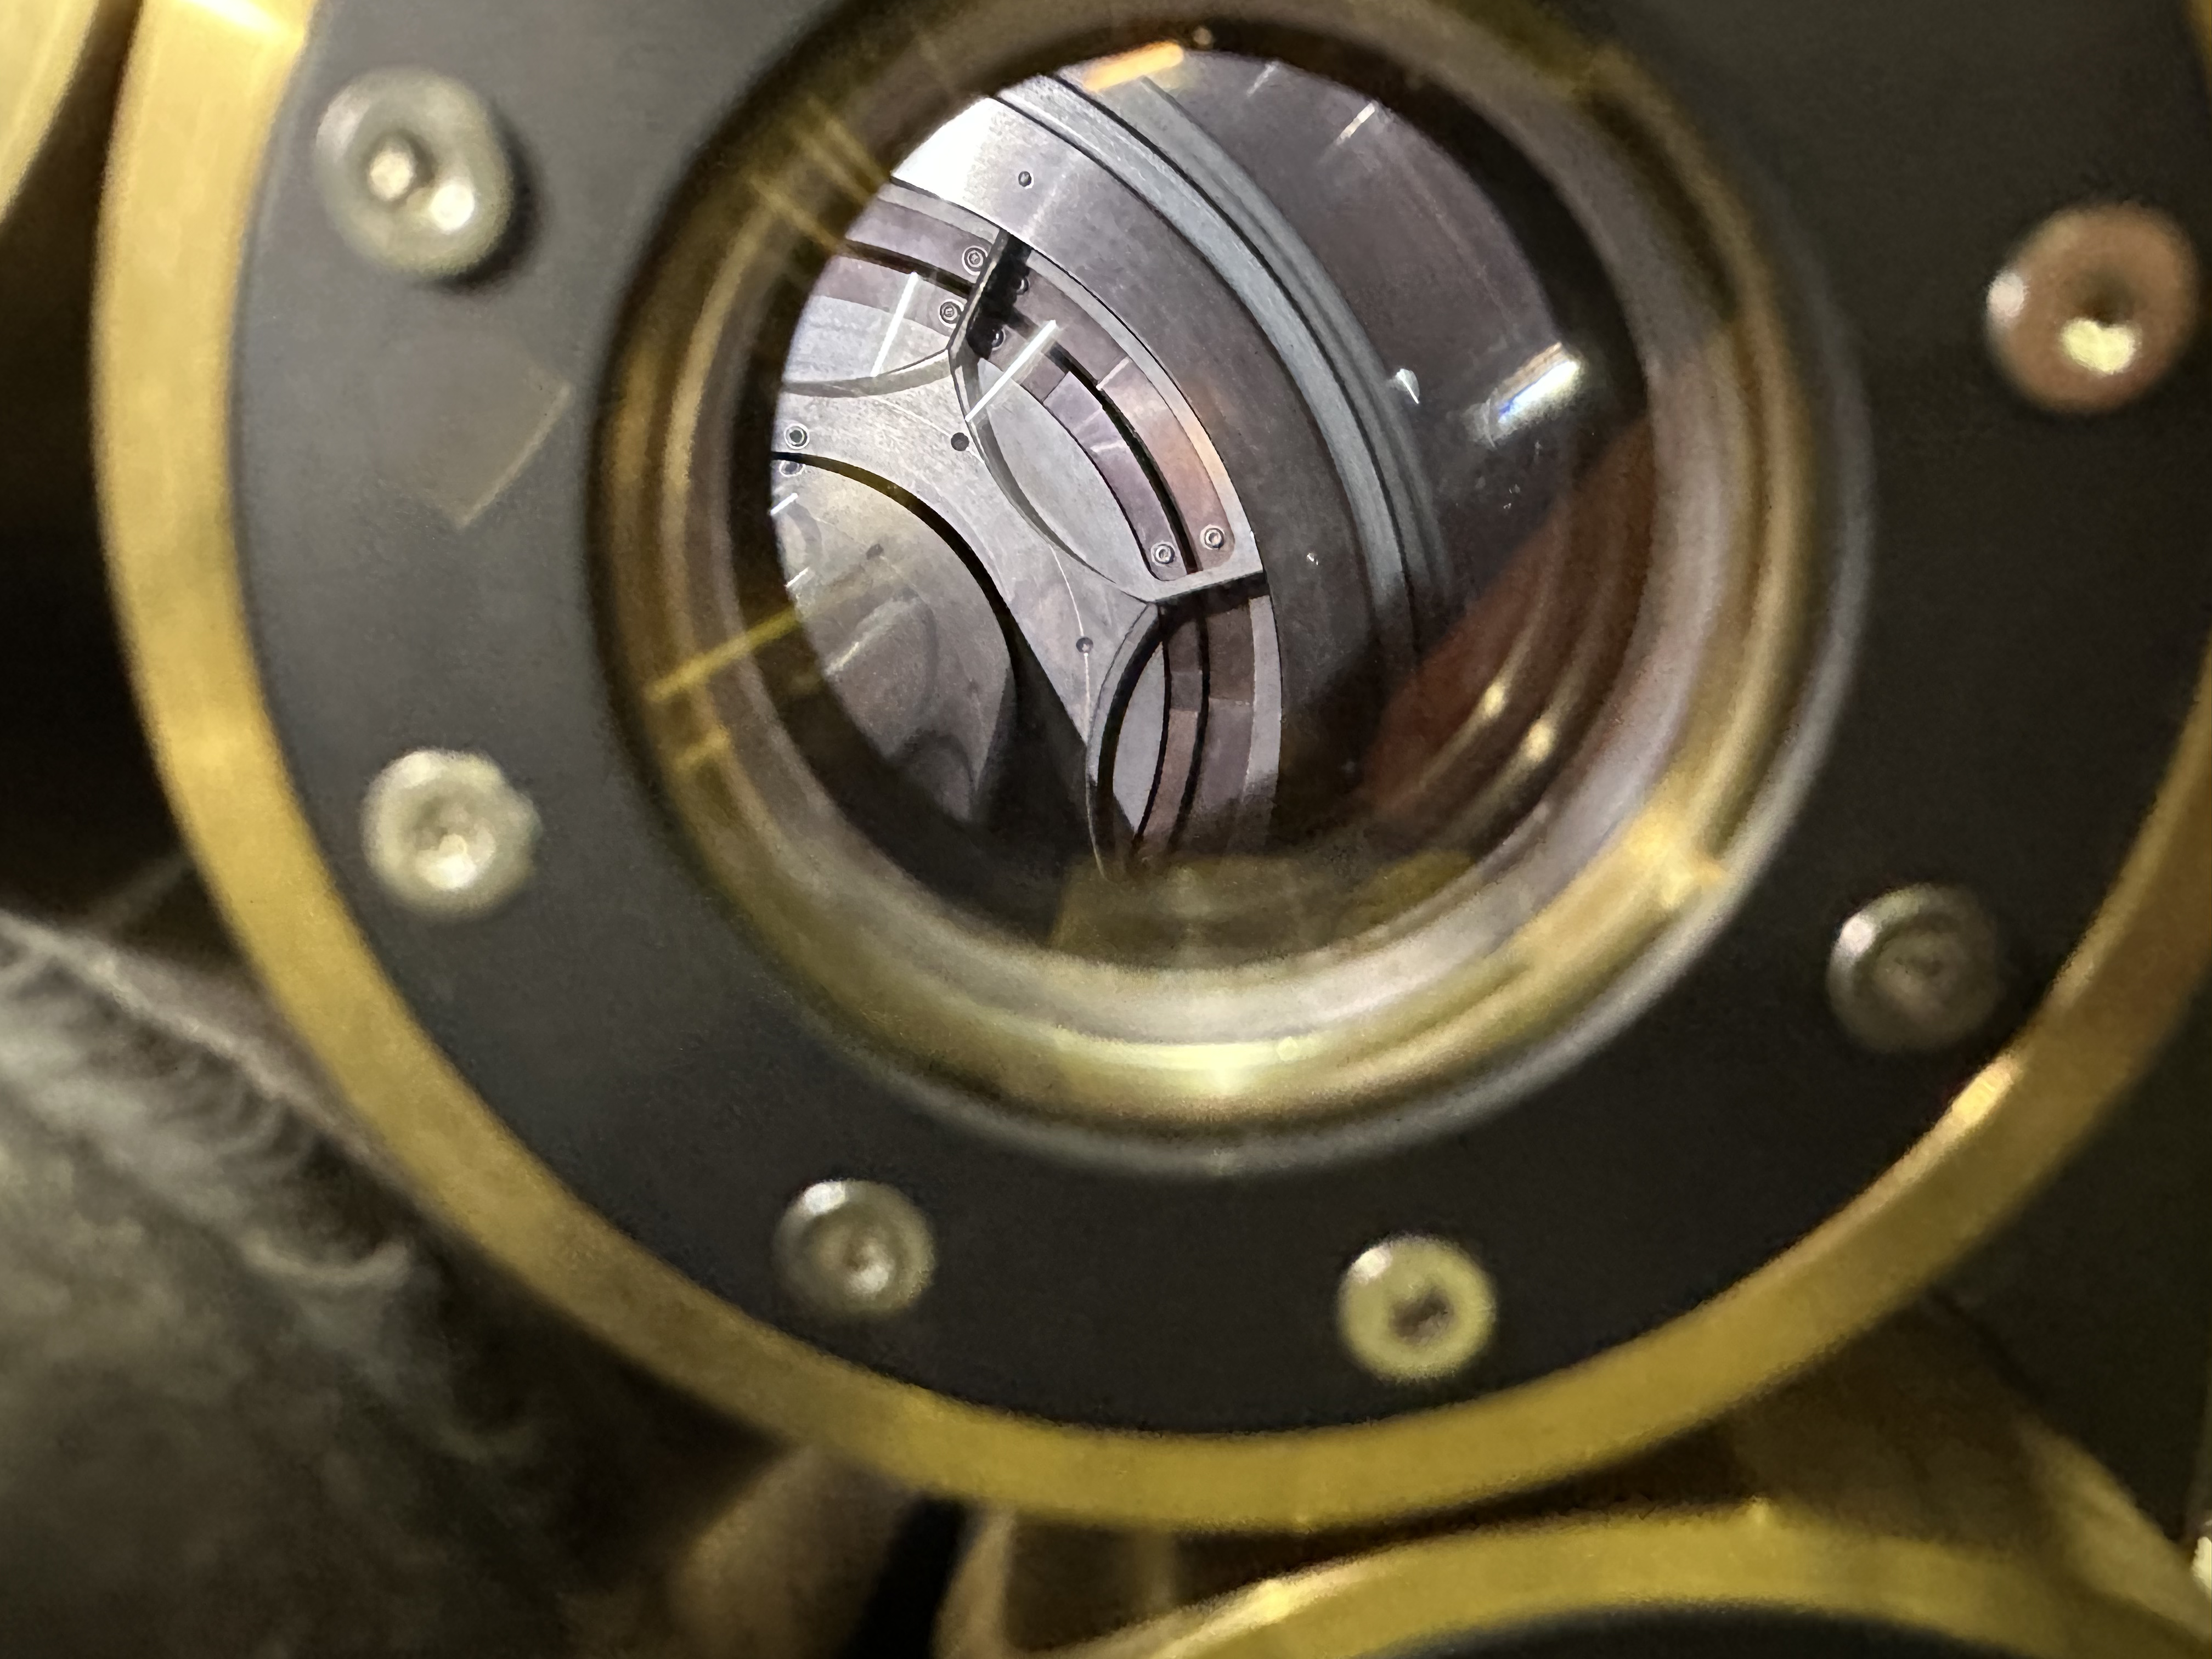
\includegraphics[height=8cm, width=0.5\textwidth]{imgs/Diaphragm_close.png} }}%
        \linespread{1.0}
        \caption{Photos showing the CEDAR diaphragm. In the left, a fully open diaphragm shown, with the nose of the CEDAR fully removed.
        In the right, a slightly open diaphragm shown through one of the quartz exit windows.}%
        \label{fig:cedarpics}%
    \end{figure}
    
    The light that passes through the aperture of the diaphragm then traverses a condenser lens (one for each aperture), designed to direct the light out of the exit windows parallel to the horizontal axis. The placement
    of the lenses are shown in Figure \ref{fig:condenser} and can be seen after the diaphragm in Figure \ref{fig:cedarpics} (right).
    \begin{figure}[t]
        \centering 
        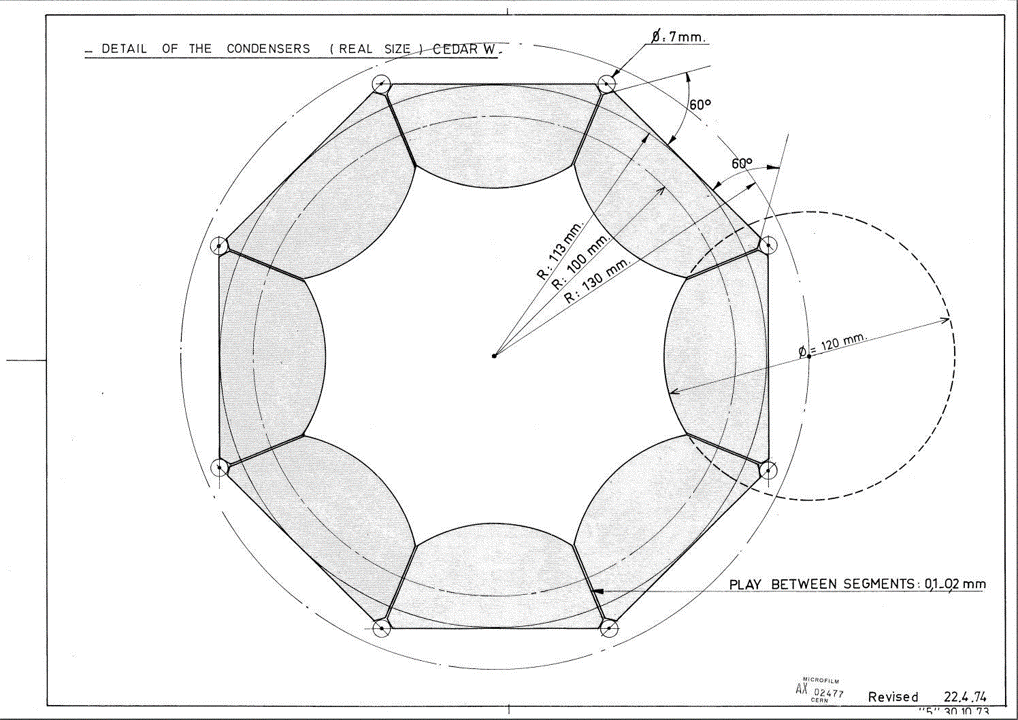
\includegraphics[width=0.8\textwidth]{imgs/Condensor_drawing.png}
        \linespread{1.0}
        \caption{Drawing showing the placement of the CEDAR condenser lenses.}
        \label{fig:condenser}
    \end{figure}
    
    The light then exits the CEDAR through eight quartz exit windows placed around the beam pipe at the upstream end of the CEDAR, shown in Figure \ref{fig:exit-windows}. Attached to the exit windows are glass filters, designed to 
    attenuate light below 240\,nm to remove light from unwanted particles.
    \begin{figure}[t]
        \centering 
        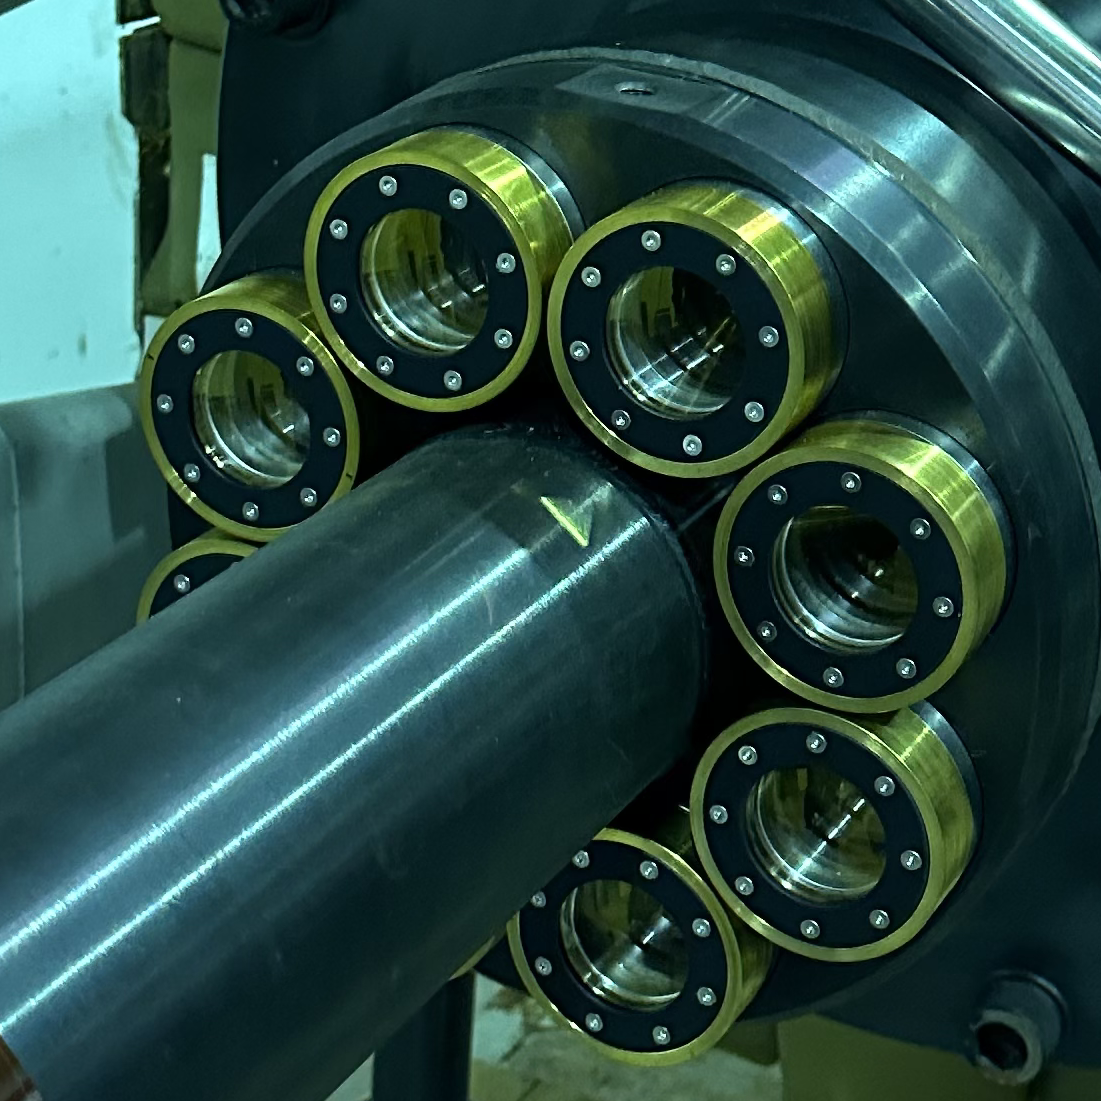
\includegraphics[width=0.5\textwidth]{imgs/exit_windows.png}
        \linespread{1.0}
        \caption{Image showing the exit windows at the upstream end of the CEDAR-W}
        \label{fig:exit-windows}
    \end{figure}

    In the original CEDAR design \cite{Bovet:1982xf}, light exiting the CEDAR through the exit windows was detected by eight ET-9820QB photomultiplier tubes (PMTs), with one attached to each window. 
    A particle was identified when there was a coincidence in at least six PMTs.
    However, this setup would not be applicable for NA62, which requires strict timming requirements on the selection of kaons of less than 100\,ps, a kaon identification efficecy of greater than 95\,\% 
    and a pion miss-identification probability of less than $10^{-4}$. To achieve these strict requirements, a purpose-built photon detection system was designed \cite{GOUDZOVSKI201586} and attached to the 
    upstream end of the CEDAR. The light exiting the quartz windows traverses through optical caps attached to the windows, which focus the light onto spherical mirrors. The spherical mirrors, one for each exit 
    window reflect the light 90 degrees into eight light boxes and boraden the light to increase the resultant light spot and are shown in Figure \ref{fig:spherical-mirror}. Each lightbox is defined as a sector 
    that will be used from now on. Each sector contains a light guid before a PMT array equipped with 48 Hamamatsu PMTs (32 of type R9880U-110 and 16 of type R7400U-03). 
    The light guide consists of a matrix of cones coated by aluminised mylar to maximise their reflectivity and direct the light onto the active area of each PMT. 
    \begin{figure}[t]
        \centering 
        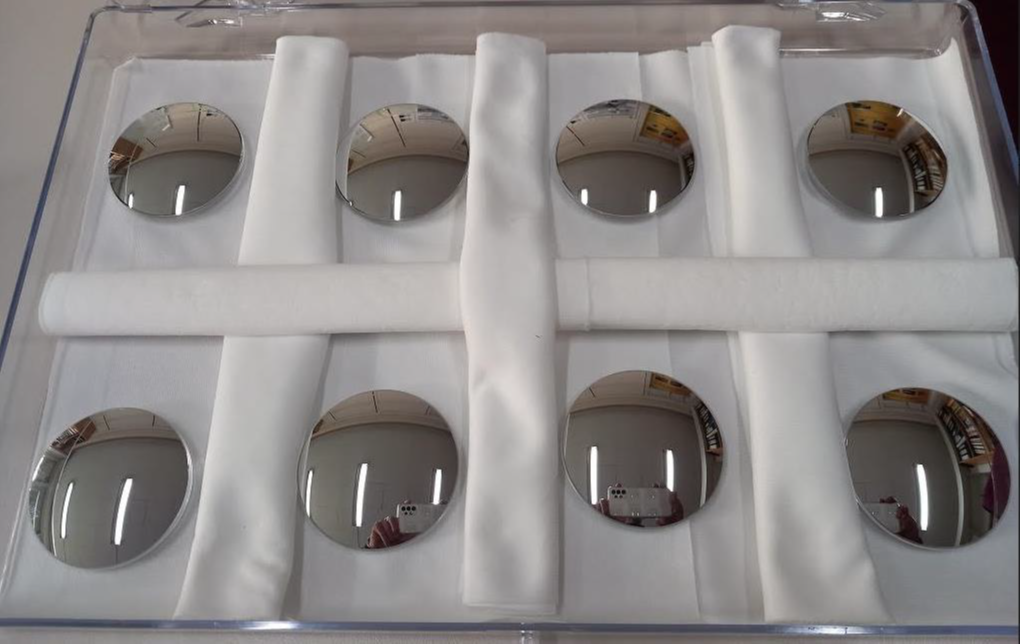
\includegraphics[width=0.5\textwidth]{imgs/spherical_mirror.png}
        \linespread{1.0}
        \caption{Image showing each of the CEDAR-H spherical mirrors, before installation into the KTAG}
        \label{fig:spherical-mirror}
    \end{figure}    
    % Explain how particles are detected
    \section{Development of CEDAR-H}
    \begin{table}[p]
        \linespread{1.0}
        \centering
        \small\caption{Optical and mechanical parameters of \CW\ and \CH. All values are dimensions in millimeters unless otherwise stated. 
        Positions along the beam axis are quoted with respect to the upstream end of the CEDAR.}
        \label{table:CedarParameterValues}
        
        \begin{tabular}{@{}llrr@{}}
        \textbf{CEDAR type} &   & \textbf{\CW} & \textbf{\CH} \\ 
        \bottomrule
        
        Nominal gas type &   & \NN & \HH \\
        \multicolumn{2}{@{}l}{Nominal pressure [bar]} & 1.71 & 3.80 \\
        \midrule
        
        \multirow{2}{*}{Gas vessel cylinder}       & Length      & 4500 & 4500 \\
        & Inner radius & 267  & 267 \\
        \midrule
        
        \multirow{2}{*}{Gas vessel cap}      & Length       & 339 & 280 \\
        & Inner radius  & 139 & 139 \\
        \midrule
        
        \multirow{5}{*}{Chromatic corrector} & Position along the beam axis& 1855 & 1902 \\
        & Radius of curvature  & 1385 & 1307 \\
        & Central thickness    & 20   & 20 \\
        & Inner radius         & 75   & 75 \\
        & Outer radius         & 160  & 160 \\
        \midrule
        
        \multirow{6}{*}{Mangin mirror}       & Position along the beam axis& 5353 & 5362 \\
        & Radius of curvature: & &  \\
        & ~~~~~~~ - refracting surface & 6615 & 8994 \\
        & ~~~~~~~ - reflecting surface & 8610 & 9770 \\
        & Central thickness                & 40   & 40 \\
        & Inner radius                     & 50   & 40 \\
        & Outer radius                     & 150  & 150 \\
        \midrule
        
        \multirow{2}{*}{Diaphragm}           & Position along the beam axis                 & 872 & 911 \\
        & Aperture central radius & 100  & 100 \\
        \midrule
        
        \multirow{3}{*}{Condensers}          & Position along the beam axis & 832 & 871 \\
        & Maximum thickness    & 10   & 10 \\
        & Radius of curvature  & 300  & 300 \\
        \midrule
        
        \multirow{4}{*}{Quartz windows}      & Position along the beam axis    & 472 & 531 \\
        & Thickness                 & 10  & 10 \\
        & Radius                    & 22.5  & 22.5 \\
        & Radial distance to window centre & 103 & 103 \\ 
        \bottomrule\bottomrule
        
        \multirow{3}{*}{Optical caps}          & Position along the beam axis & 450 & 450 \\
        & Maximum thickness    & 4.24   & 4.24 \\
        & Radius of curvature  & 114.62  & 114.62 \\
        \midrule
        
        \multirow{5}{*}{Spherical mirrors}   & Position along the beam axis             & 322 & 322 \\
        & Radius of curvature           & 51.68 & 77.52\\
        & Diameter                      & 50  & 50 \\
        & Radial distance to mirror centre & 106 & 106 \\ 
        \end{tabular}
        
    \end{table}
        
    \begin{figure}[t]
        \centering 
        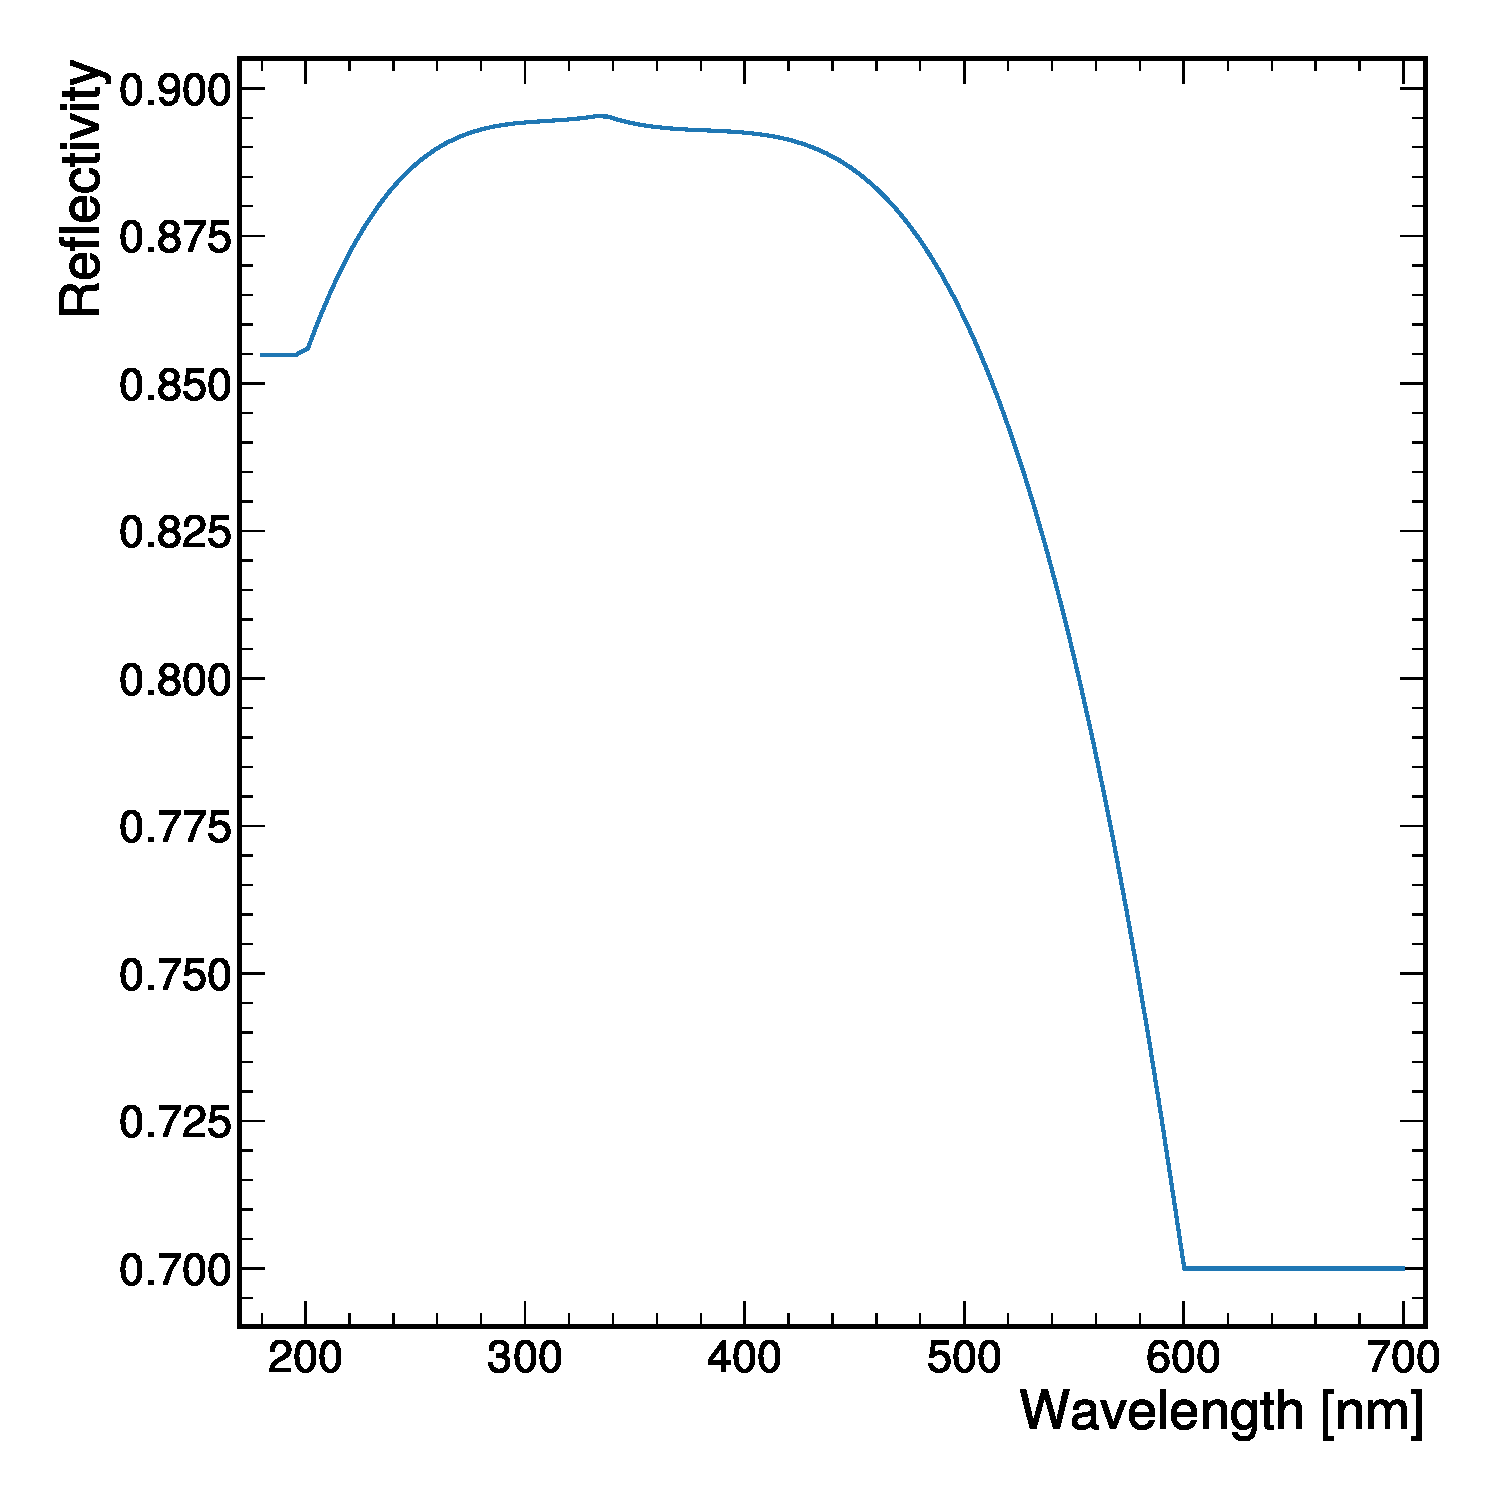
\includegraphics[width=0.8\textwidth]{plots/ManginReflec.pdf}
        \linespread{1.0}
        \caption{Meausured reflectivity of CEDAR-H mangin mirror conducted by Winlight System}
        \label{fig:ManginReflec}
    \end{figure}

    \begin{figure}[t]
        \centering 
        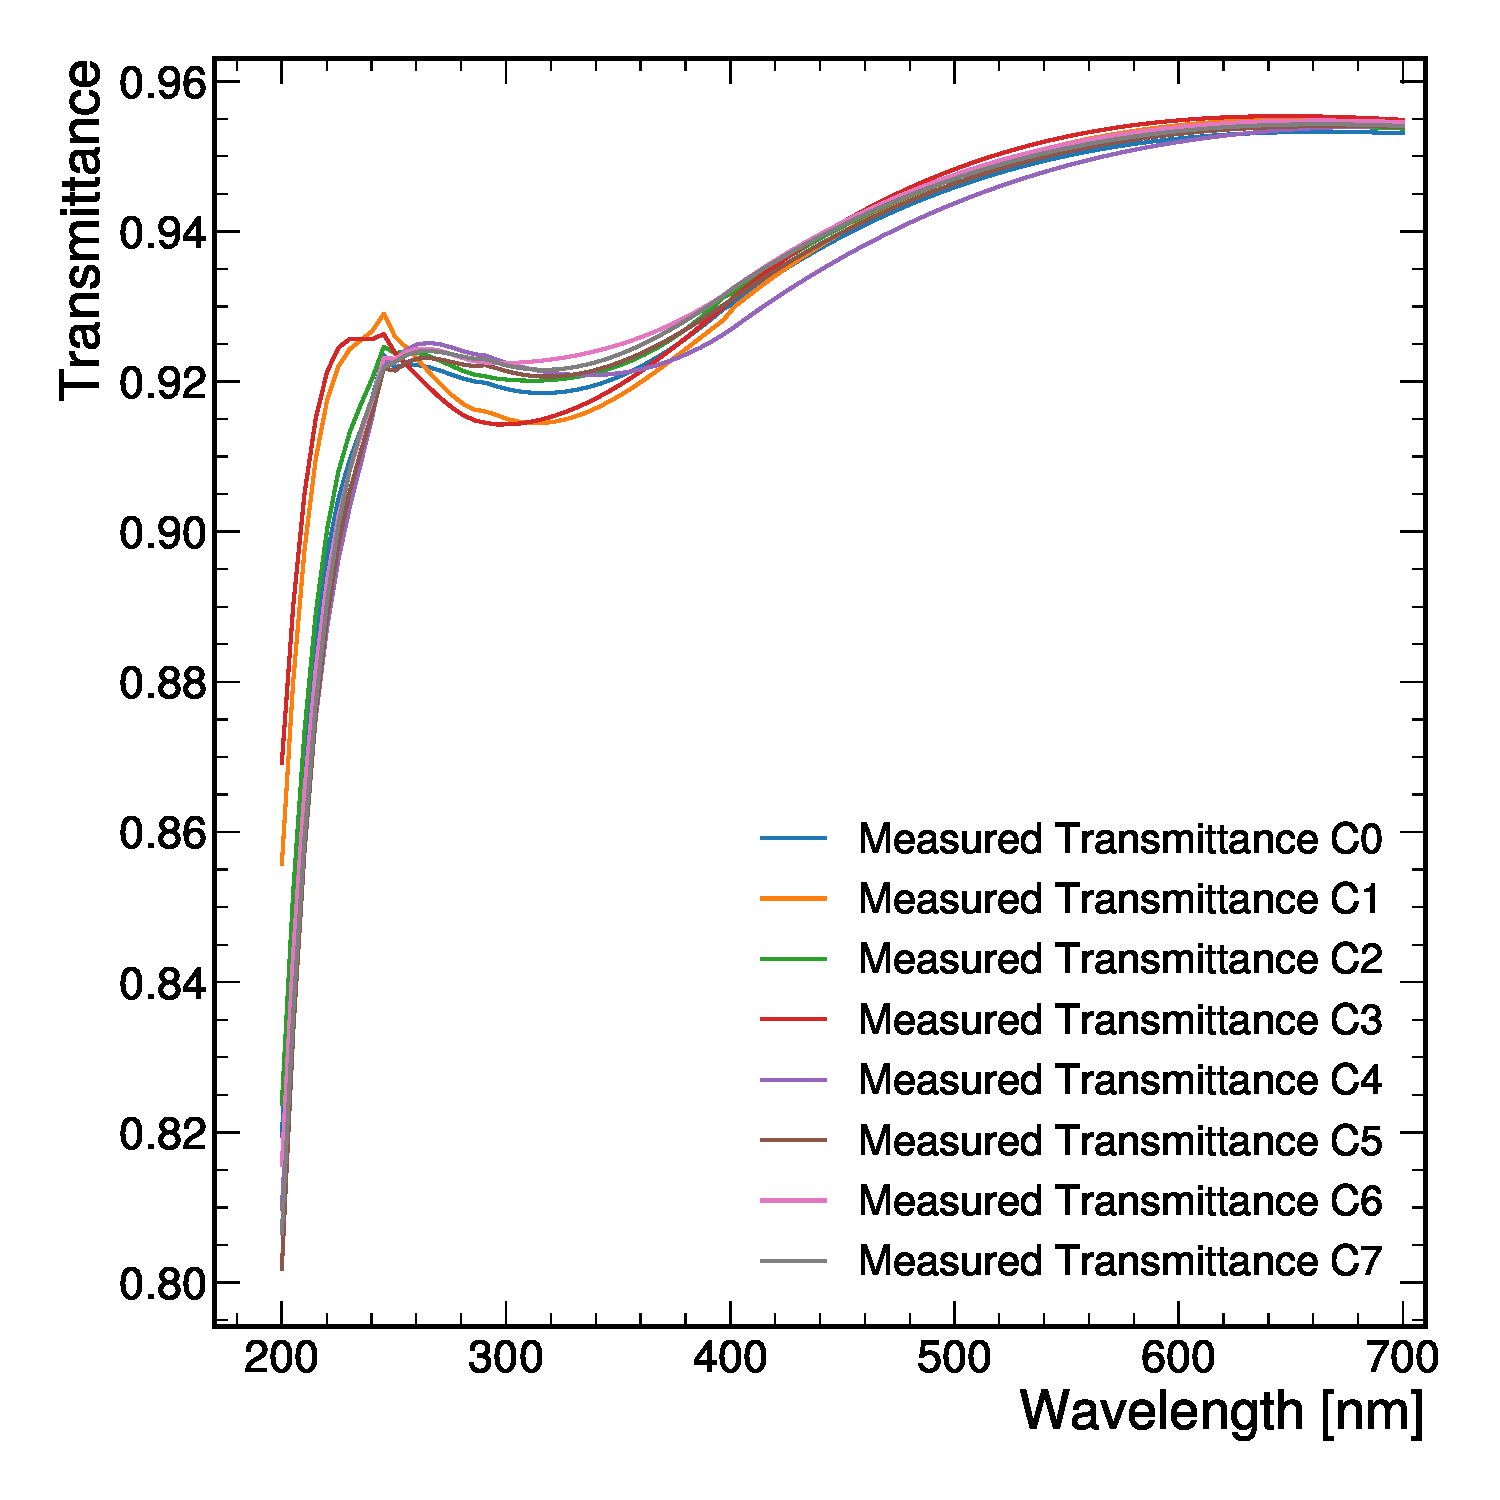
\includegraphics[width=0.8\textwidth]{plots/TranmitCL.pdf}
        \linespread{1.0}
        \caption{Meausured transmittance of CEDAR-H condenser lenses conducted by Thomas Schneider at CERN}
        \label{fig:CLTransmit}
    \end{figure}

    \begin{figure}[t]
        \centering 
        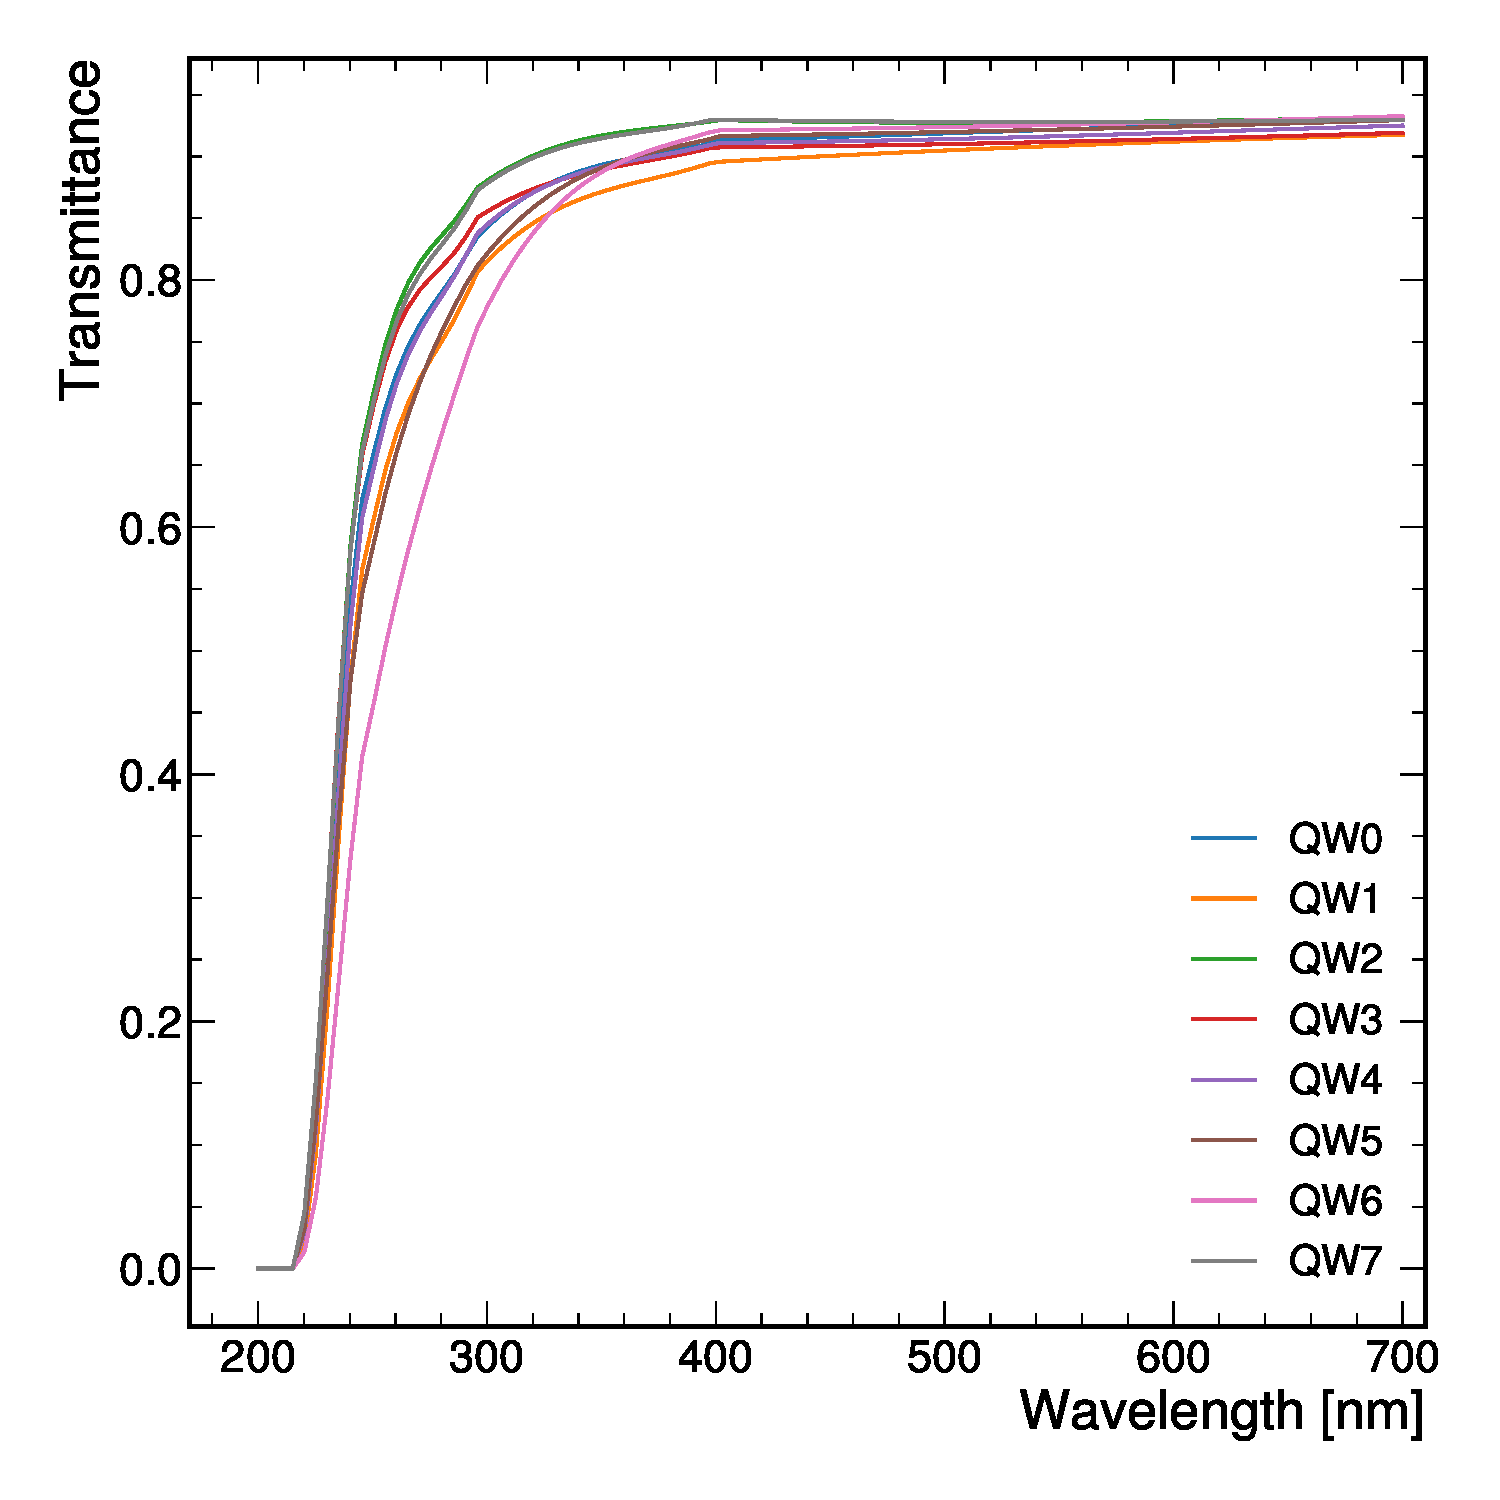
\includegraphics[width=0.8\textwidth]{plots/TranmitQW.pdf}
        \linespread{1.0}
        \caption{Meausured transmittance of CEDAR-H quartz lenses conducted by Thomas Schneider at CERN}
        \label{fig:QWTransmit}
    \end{figure}

    \begin{figure}[t]
        \centering 
        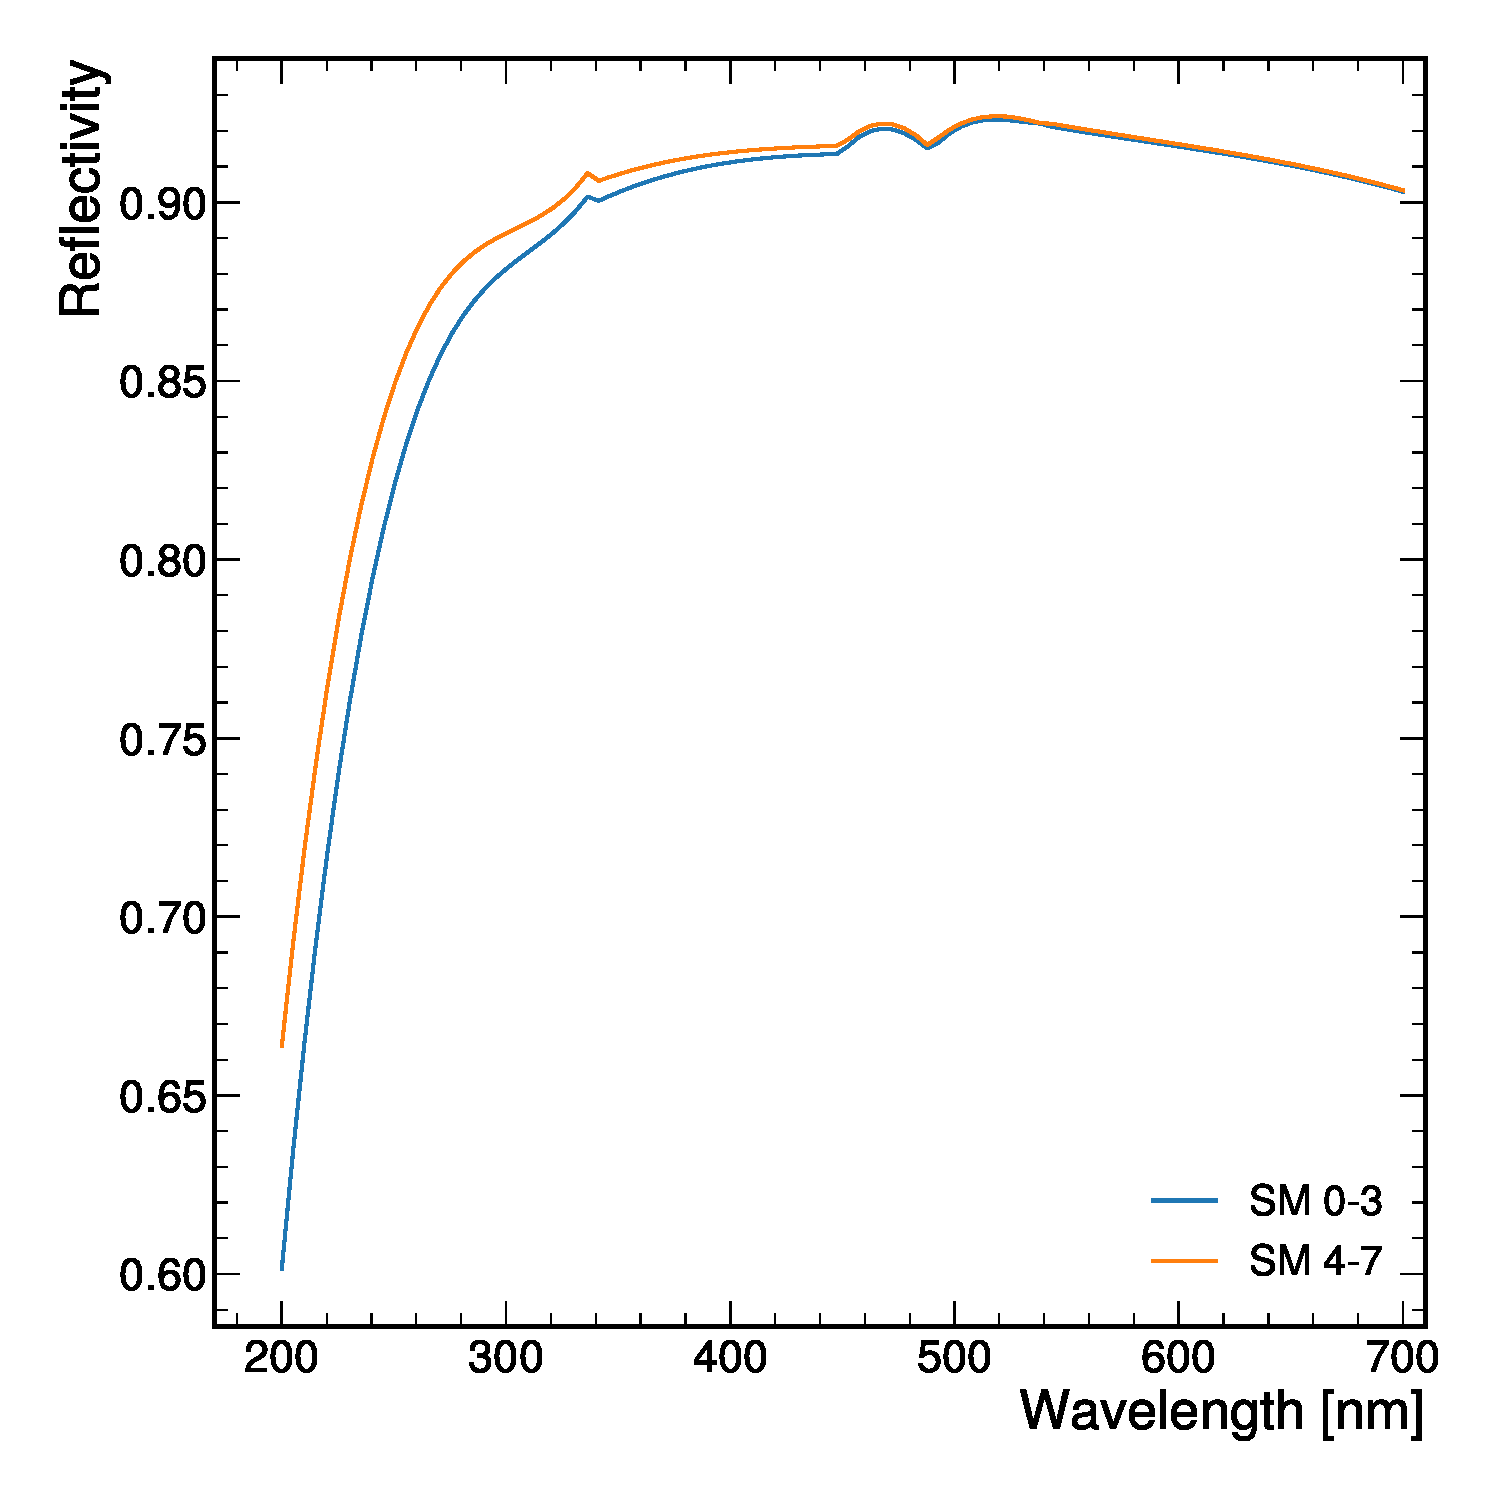
\includegraphics[width=0.8\textwidth]{plots/ReflectivitySM.pdf}
        \linespread{1.0}
        \caption{Meausured reflectivity of KTAG spherical mirror conducted by Thomas Schneider at CERN}
        \label{fig:CLTransmit}
    \end{figure}


    \section{Test-beam at CERN}

    \section{Comissioning at CERN}

    \section{CEDAR-H Performance at NA62}

    \ifSubfilesClassLoaded{%
        \bibliographystyle{IEEEtran}
        \bibliography{../../../references.bib}%
    }{} 
\end{document}